\documentclass[12pt]{article}
\usepackage[utf8]{inputenc}      % For UTF-8 support
\usepackage[T1]{fontenc}
\usepackage{lmodern}
\usepackage{geometry}
\usepackage{booktabs}            % For nicer tables
\usepackage{hyperref}            % For hyperlinks in the document
\usepackage{graphicx}            % For images
\usepackage{array}               % For extended table features
\usepackage{setspace}
\usepackage{csquotes}
\usepackage[backend=biber, style=ieee]{biblatex}
\addbibresource{bibliography.bib}
\usepackage{helvet}
\renewcommand{\familydefault}{\sfdefault}
\geometry{margin=1in}
\setstretch{1.15}
\usepackage{placeins}
\usepackage{float}

\begin{document}

\begin{titlepage}
  \centering
  \vspace*{1in}
  {\Huge\bfseries Used Car Characteristics\par}
  \vspace{0.5em}
  {\Large An Exploratory and Predictive Data Analysis\par}
  \vspace{1.5in}
  {\Large Dávid Fodor \\ Faisal Zayeem Khan \\ Márió Palágyi\par}
  \vfill
  {\large Submission date: \textit{25.06.2025}\par}
  \vspace{0.5in}
  {\large Datascience Capstone Project - IMC Krems}
\end{titlepage}

\begin{abstract}
This project addresses the complex challenge of accurately predicting used car prices by developing a robust machine learning model. Utilizing a comprehensive dataset scraped from a major European online car marketplace, we conducted extensive data preprocessing and feature engineering. A key focus was placed on transforming complex, semi-structured text features—such as optional extras and convenience packages—into a structured format suitable for modeling. We evaluated several regression algorithms, including Random Forest and Neural Networks, ultimately selecting XGBoost for its superior performance. Through iterative hyperparameter tuning and meticulous feature engineering, our final model achieved a high predictive accuracy, with a Mean Absolute Error (MAE) of €1735.70 and an R-squared value of 0.9496 and MAPE of \textit{16.34\%} on the test set, making predictions in the \textit{0 - 60k} euros range. The results demonstrate that detailed feature extraction from composite text fields, combined with a powerful gradient boosting framework, can create a highly effective and reliable model for vehicle price prediction, significantly outperforming baseline approaches, however our results also suggest that the most important step by far is having the right data and proper cleaning. We have also gathered feature importances for multiple models, concluding that the base numerical descriptors like mileage and power combined with the car's make and model are the most important features as expected. Through a surface level literature review, we have found that while papers in this topic are numerous, they are not as usefull as one might think due to common lacking description and disclosure of the data pipeline.
\end{abstract}

\vfill

\textbf{Individual contributions:}
\begin{itemize}
  \item \textbf{Dávid Fodor:} \textit{60\%} - Data Scraping, Preprocessing, EDA, Predictions, Literature Review, Report Writing, Presentations
  \item \textbf{Faisal Zayeem Khan:} \textit{20\%} - EDA, Presentations
  \item \textbf{Márió Palágyi:} \textit{20\%} - EDA, Presentations
\end{itemize}

\vspace{1em}
\href{https://github.com/dfoddav2/SS25-capstone-project}{Public repository with data available here}.

\vspace{2em}
\textit{Note: This document is a condensed summary of our work. For a comprehensive discussion, detailed experimental results, and in-depth analysis, please refer to the full technical report.}

\newpage
\tableofcontents

\newpage
\section{Introduction}

The used car market is a complex environment where pricing is often opaque, making it difficult for both buyers and sellers to determine a fair value. This project was motivated by a desire to bring transparency to this market by leveraging data science. We embarked on a large-scale web scraping effort to build a unique dataset and explore the factors that influence used car prices.

Our primary research questions were:
\begin{itemize}
  \item What features significantly influence the price of a used car?
  \item Is it possible to build a model that accurately predicts used car prices from these features?
\end{itemize}

The goal was to move beyond simple exploration and develop a predictive model with practical applications, such as a price suggestion tool for online marketplaces. This report summarizes our journey from data collection to the final, highly accurate prediction model.

\newpage
\section{Methodology}

Our project followed a standard data science workflow, from data acquisition and cleaning to modeling and evaluation.

\begin{figure}[H]
  \centering
  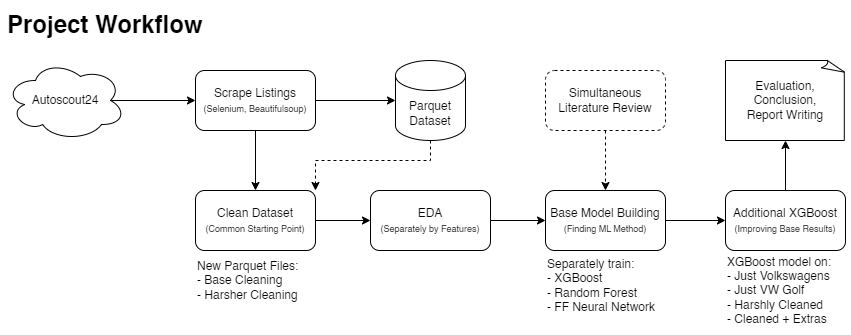
\includegraphics[width=0.9\textwidth]{./images/project_flow.png}
  \caption{Project Flow. Source: Own work}
  \label{fig:project_flow}
\end{figure}

\subsection{Data Collection \& Preprocessing}

We scraped over 500,000 car listings from \url{https://www.autoscout24.com/}, a major European marketplace. The initial dataset was noisy and required extensive cleaning. Key preprocessing steps included:
\begin{itemize}
    \item \textbf{Feature Engineering:} Transforming raw data like registration\_date into a usable age\_months feature.
    \item \textbf{Imputation:} Intelligently filling missing values based on other features (e.g., setting age\_months to 0 for cars listed as New).
    \item \textbf{Outlier Removal:} We applied two main cleaning strategies. A standard cleaning pass removed clear errors and extreme outliers. A second, harsh cleaning pass was designed to create a more uniform dataset focused on the most common market segment (prices up to approx. €64k), which proved crucial for model performance. This harsh cleaning removed an additional 32\% of the data but significantly improved model accuracy.
\end{itemize}

\begin{figure}[H]
  \centering
  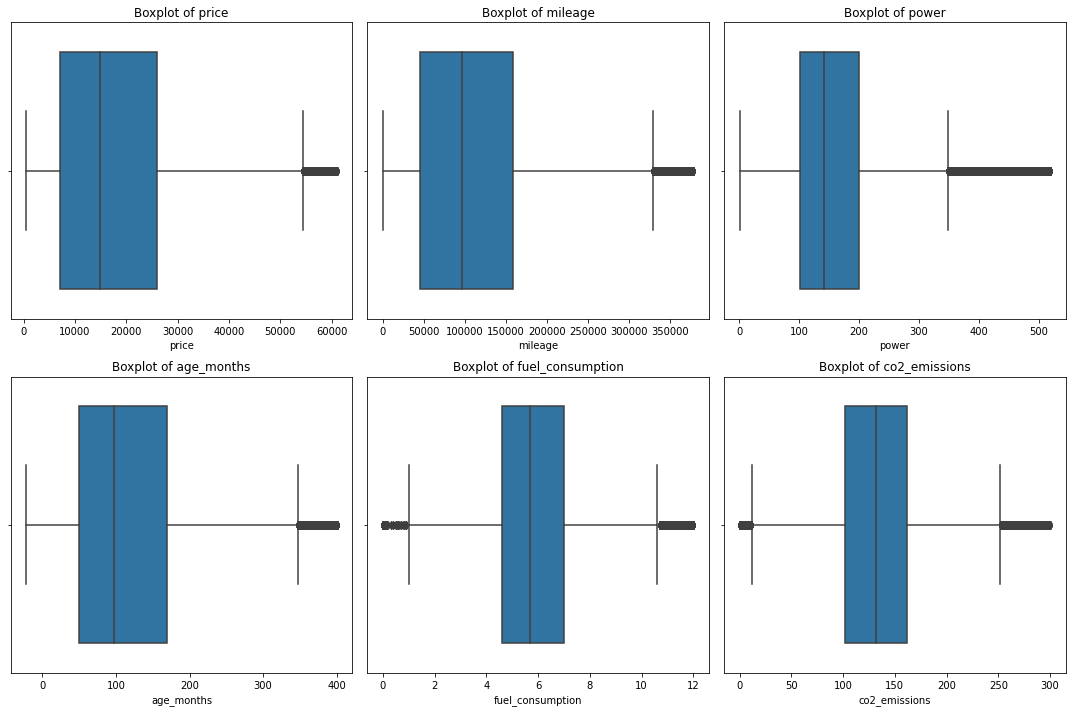
\includegraphics[width=0.8\textwidth]{./images/boxplots_harshly_cleaned.png}
  \caption{Boxplots of Numerical Features After Harsh Cleaning. Source: Own work}
  \label{fig:boxplots_after_harsh}
\end{figure}

\subsection{Exploratory Data Analysis (EDA)}
Our EDA revealed strong correlations between price and features like `power`, `age\_months` (negative), and `mileage` (negative), as expected. We also uncovered interesting patterns related to seller type, country of sale, and the prevalence of optional extras. This exploration confirmed that our dataset was rich enough for predictive modeling.

\newpage
\section{Results}

We experimented with several models, including Random Forest, Neural Networks, and XGBoost. While initial models trained on the broadly cleaned dataset performed adequately (R² = 0.79), their Mean Absolute Error (MAE) was too high for practical use (about €30,000).

The key breakthrough came from training models on the "harshly cleaned" dataset, which focused on the core of the used car market. This strategy dramatically improved performance across all metrics. Our final and best-performing model was an XGBoost Regressor trained on this dataset, further enhanced with engineered features from text descriptions of optional extras.

\begin{table}[H]
  \centering
  \begin{tabular}{@{}lcc@{}}
    \toprule
    \textbf{Final Model Metrics} & \textbf{Train} & \textbf{Test} \\
    \midrule
    Mean Absolute Error (MAE) & 1212.67 & 1735.70 \\
    R-squared (R\textsuperscript{2}) & 0.9835 & 0.9496 \\
    Mean Absolute Percentage Error (MAPE) & 12.79\% & 16.34\% \\
    \bottomrule
  \end{tabular}
  \caption{XGBoost Results on Harshly Cleaned Dataset with Extra Features}
  \label{tab:xgboost_harshly_cleaned_extra_features_results}
\end{table}

This model achieved an R² of \textbf{0.9496} and an MAE of just \textbf{€1735.70} on the test set, a result that is both statistically significant and practically useful.

\begin{figure}[H]
  \centering
  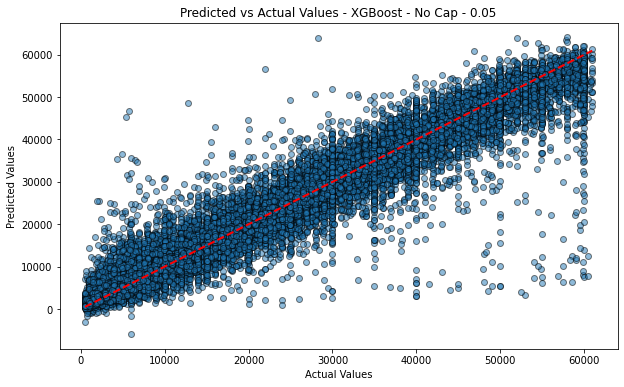
\includegraphics[width=0.8\textwidth]{./images/extras_harshly_cleaned_predicted_vs_actuals.png}
  \caption{Predicted vs Actual Prices for the Final Model. Source: Own work}
  \label{fig:predicted_vs_actual_harshly_cleaned_extra_features}
\end{figure}

Feature importance analysis of the final model confirmed that `power`, `age\_months`, and `mileage` were the top predictors, but also highlighted the impact of specific features like `use\_type` (New, Used, etc.) and certain high-value optional extras.

\begin{figure}[H]
  \centering
  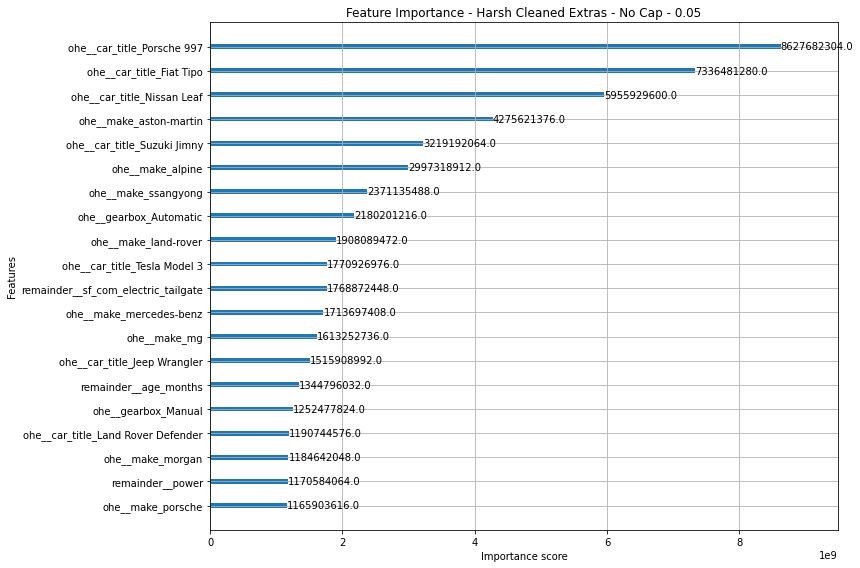
\includegraphics[width=0.8\textwidth]{./images/extras_harshly_cleaned_feature_importance.png}
  \caption{Top 20 Feature Importances for the Final Model. Source: Own work}
  \label{fig:feature_importance_harshly_cleaned_extra_features}
\end{figure}

\newpage
\section{Discussion \& Conclusion}

Our work leads to three main conclusions:
\begin{enumerate}
    \item \textbf{Data is King:} The single most important factor for achieving high accuracy was not the choice of a complex algorithm, but rather the meticulous and strategic cleaning of the dataset. A general model for all cars is impractical; focusing on a well-defined market segment is essential.
    \item \textbf{A Practical Model is Achievable:} With the right data strategy, it is possible to build a highly accurate price prediction model (R² > 0.94) with a practically low error rate (MAE < €1800), suitable for real-world applications.
    \item \textbf{Feature Engineering Adds Value:} While core features like power and age are dominant, systematically extracting and including data from text descriptions (like optional extras) provides a measurable improvement in model performance.
\end{enumerate}

In conclusion, this project successfully navigated the entire data science pipeline to answer our research questions. We demonstrated that by combining a large, custom-scraped dataset with rigorous preprocessing and a powerful XGBoost model, one can create a reliable and accurate tool for predicting used car prices. Future work could explore building an ensemble of specialized models for different market segments (e.g., luxury, budget, electric) to provide comprehensive coverage of the entire market.

\newpage
\FloatBarrier
\section{Bibliography}
\printbibliography[heading=none]

\end{document}